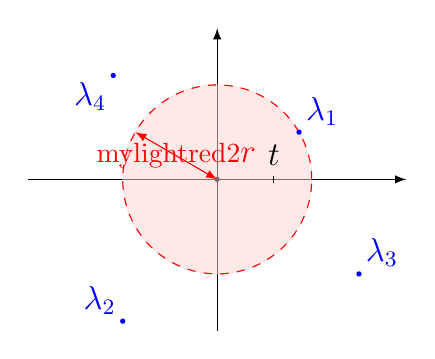
\begin{tikzpicture}[scale=1.2]
  \definecolor{mylightred}{RGB}{255,210,210}
  \definecolor{myred}{RGB}{255,0,0}
  \definecolor{mylightred2}{RGB}{255,232,232}
      \def\ang{150}
      \def\R{1}
      \coordinate (O)  at (0, 0);
      \coordinate (L1) at (30:1);
      \coordinate (L2) at (-1, -1.5);
      \coordinate (L3) at (1.5, -1);
      \coordinate (L4) at (1.2, 1);
      \coordinate (L5) at (-1.1, 1.1);
     
      \draw[-latex] (0, -1.6) -- (0, 1.6);
      \draw[-latex] (-2, 0) -- (2, 0);
      \fill[radius=0.8pt,black] (O) circle;
      \draw[mylightred, fill, opacity=0.5] (O) circle (\R);
      \draw[myred, dashed] (O) circle (\R);
      \fill[radius=0.8pt,blue]
        (L1) circle node[above right=-1pt] {\large $\lambda_1$}
        (L2) circle node[above left =-1pt] {\large $\lambda_2$}
        (L3) circle node[above right=-1pt] {\large $\lambda_3$}
        (L5) circle node[below left =-1pt] {\large $\lambda_4$};
      \draw (0.6, -0.04) -- (0.6, 0.04)  node[above] {\large $t$};
      \draw[latex-latex, myred] (O) -- (\ang:\R) node[midway] {\contour{mylightred2}{\large $r$}};
\end{tikzpicture}